% Submission draft. The author's affiliation and corresponding-author contact remain to be supplied.
% EAB title and layout follow the supplied manuscript examples.
\documentclass[conference]{IEEEtran}
\usepackage[T1]{fontenc}
\usepackage{amsmath,amssymb,booktabs,multirow,xcolor,url,tabularx,array}
\usepackage{graphicx}
\title{[Experiment, Analysis, and Benchmark] Evaluating Language Models and Subspace Methods for Explaining Known Tabular Outliers}
\author{\IEEEauthorblockN{Lili Guan}\\
\IEEEauthorblockA{ORCID: \url{https://orcid.org/0000-0002-4464-9384}}}
\begin{document}
\maketitle

\begin{abstract}
Tabular anomaly detectors flag suspicious rows but do not identify which attributes an analyst should inspect. We study known-outlier explanation: given a flagged row, its schema, and a finite sample of normal rows, rank feature subsets that distinguish it from the clean population. Evaluation is difficult because existing resources rarely provide minimal feature-level labels, while a small reference sample can make unnecessary subsets appear sufficient. We introduce a procedural benchmark with exhaustively enumerated clean populations, template-disjoint splits, and separate labels for population support, rule sufficiency, mechanism, and hidden edits. We compare three local language models with mixed-type subspace rankers and controls, using separate measures of sufficiency, exact minimal-set recovery, ranked retrieval, compactness, and output validity. Across 864 test cases, reference-sample minimal sets matched population-minimal labels in only 2 cases. In a separate 288-case field-order test, randomization reduced the three language models' localization scores by 0.076--0.202. On the main benchmark, Qwen led non-control methods on support sufficiency@1 (0.714), while Gower-LOF achieved the highest exact@1 (0.517), Hit@4 (0.634), and best Jaccard@4 (0.759). Circuit evaluation uses fault-specific labels; the 78-query real-table pilot measures peer agreement, not accuracy. These results show that conclusions depend on both the explanation target and the available evidence. The study covers one generator and two small external pilots.
\end{abstract}

\begin{IEEEkeywords}
data quality, anomaly explanation, feature subspaces, large language models, benchmark evaluation
\end{IEEEkeywords}

\section{Introduction}
An anomaly detector flags a suspicious row, but a data analyst still needs to determine which attributes deserve inspection. This is a common step in data-quality review: the row-level decision narrows the search to one record, while the explanation must identify a useful subset of its fields. Figure~\ref{fig:intro-sample-gap} illustrates this setting with an actual query from the Pima table in ADBench~\cite{han2022adbench}.

\textbf{A real-table example.} The target is row 259, with glucose 155 and body-mass index (BMI) 33.3. All five models receive its eight values under opaque feature IDs and the same 12 normal reference rows. In the recorded response, Qwen ranks F007, F002, and F001; the other models' strict-majority set is \{F001, F002, F005\}, giving Jaccard agreement 0.500. Thus, a shared row and reference sample can produce different field selections. The plot provides context, while the recorded outputs expose the evaluation question: which selection is a valid explanation? The row label alone cannot answer it, because Pima has no trusted feature-level labels in this pilot.

\begin{figure*}[t]
\centering
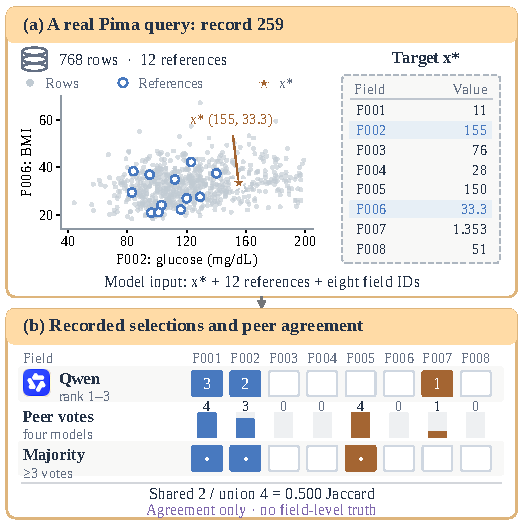
\includegraphics[width=\textwidth]{figures/figure_intro_real_dataset.pdf}
\caption{A recorded Pima query and its explanation disagreement. (a) Glucose and BMI from the 768-row ADBench table, with target row 259 marked by a star and its 12 supplied references outlined; rows with zero glucose or BMI are omitted from the projection. (b) A slice of the actual model-visible rows, Qwen's recorded ranking, and the strict-majority feature set of its four peers. All eight fields and 12 references are supplied in the query. Row IDs, class labels, and the semantic axis names are for illustration only; the model sees opaque feature IDs. The example measures agreement and provides no clinical or feature-level ground truth.}
\label{fig:intro-sample-gap}
\end{figure*}

We study explanation after detection, not the detector itself. Given a known outlier $x^*$, its schema, and a finite sample of normal reference rows, a method returns ranked feature subsets. The input contains neither a detector score nor the paired clean row. The task is therefore a data-centered description of a supplied outlier; it does not explain a detector's score, recommend a repair, or establish causality~\cite{li2024xadsurvey}. Our evaluation measures feature localization and ranking.

\textbf{Evaluation challenges.} Related work calls these tasks anomaly explanation, outlier interpretation, or outlier description~\cite{panjei2022survey,li2024xadsurvey}. Yet existing evaluation resources leave three gaps. First, tabular benchmarks commonly label anomalous rows or data-quality errors, but rarely provide minimal feature-level explanations for each known outlier~\cite{choudhury2025tabard,gu2025radar,han2022adbench}; circuit studies provide such labels only for a narrow gate-negation setting~\cite{antwarg2024groundtruth}. Second, the target explanation may be defined over the full clean population even though a method sees only a sample. A clean pattern omitted by sampling can make an unnecessary field appear sufficient. Third, sufficiency alone rewards broad answers: selecting every field guarantees sufficiency but provides little localization. A useful benchmark must therefore measure sufficiency, minimal recovery, ranked retrieval, and output validity separately.

These gaps motivate three questions: How much reference evidence is needed to recover a population-level explanation? How should broad but sufficient answers be compared with concise minimal ones? What claims are supported by synthetic labels, circuit labels, and real-table peer agreement? We address these questions with an evaluation benchmark, not a new detector or explainer.

\textbf{Our study.} Our benchmark makes each question measurable. It exhaustively enumerates finite clean populations, separates train/development/test sets by rule template, and labels population support, rule sufficiency, anomaly mechanism, and hidden edits separately. We compare three local language models with transparent controls and mixed-type subspace rankers, then test sensitivity to field order. Two external pilots extend the analysis: a digital-circuit track with fault-specific feature labels and a real-table track that measures leave-one-model-out agreement. We report each track separately because their labels support different claims.

This paper makes four contributions:
\begin{itemize}
  \item \textbf{Task and labels.} We formalize known-outlier explanation and distinguish population support, rule sufficiency, mechanism, and edit provenance.
  \item \textbf{Benchmark.} We provide exhaustively labeled clean populations, 40 rule templates, template-disjoint splits, and three seed-specific test runs.
  \item \textbf{Comparative analysis.} We evaluate language models, mixed-type rankers, and controls with separate localization and validity measures. The results quantify finite-reference ambiguity and field-order sensitivity.
  \item \textbf{Scoped external pilots.} We add circuit and real-table evaluations, interpreting the first as fault-specific localization and the second as peer agreement only.
\end{itemize}


\section{Task and Label Semantics}
Let $T$ be a table with feature set $F=\{f_1,\dots,f_d\}$, let $x^*$ be a known outlier, and let $R$ be the supplied normal reference sample. A method returns up to $K$ ranked subsets,
\[
  \widehat{\mathcal{E}}(x^*,R,T)=(S_1,\ldots,S_K), \qquad S_k\subseteq F,
\]
with optional evidence text, confidence, or abstention. We evaluate which fields describe the known outlier, not whether a detector can find it. Because no detector score is provided, the task is data-centered; it does not measure how faithfully an explanation represents an upstream model~\cite{li2024xadsurvey}.

We keep five kinds of labels separate. $M_{\mathrm{direct}}$ marks fields changed from a hidden clean row; $M_{\mathrm{value}}$ marks fields whose values changed, including propagated changes; and $M_{\mathrm{rule}}$ marks fields that can affect the generator's anomaly rule. $\mathcal{S}_{\mathrm{support}}^{\min}$ contains the smallest-by-inclusion subsets whose target values never occur in the clean population. $\mathcal{S}_{\mathrm{rule}}^{\min}$ contains the smallest-by-inclusion subsets that are enough to establish the generator's rule. These sets can differ, and a minimal set need not have the fewest fields among all valid explanations.

The prompt does not show the paired clean row, so direct edits are hidden and are not a prediction target. Our primary target is descriptive: whether a feature subset identifies values absent from the clean population. It is not a causal explanation. We score rule-related labels separately on generated data. On real data, where feature-level truth is unavailable, we report peer-model agreement only.

The target label is defined from the full clean population, but a method sees only $R$. A feature pattern absent from the full population must also be absent from $R$; however, sampling may make other patterns appear absent. Thus a subset that looks minimal in $R$ may not be minimal in the population. We retain the population-level label and separately measure this ambiguity in the reference sample.

Formally, let $P_X$ be the clean population and let $\pi_S$ keep only the fields in subset $S$. $S$ is support-sufficient if the target projection $\pi_S(x^*)$ never occurs in $P_X$. For our finite synthetic data, we enumerate the population and test this exactly. $S$ is rule-sufficient if every full row that matches $x^*$ on $S$ satisfies the generator's rule; it is rule-minimal if no proper subset has this property. Support-minimality is defined in the same way. Minimality is by set inclusion, so two minimal explanations can have different sizes. These labels answer different questions and are not combined:

For a rule $A(f_1)\lor B(f_2)$, if both parts hold, either singleton $\{f_1\}$ or $\{f_2\}$ is sufficient; their union is sufficient but not minimal. Likewise, an edit to $f_3$ may change a proxy field $f_4$, while the rule depends only on $f_4$. Then the directly edited, value-changed, and rule-related fields differ. These examples show why one feature-level score cannot represent all targets. They are schematic and make no causal claim about real tables.

\begin{figure*}[t]
\centering
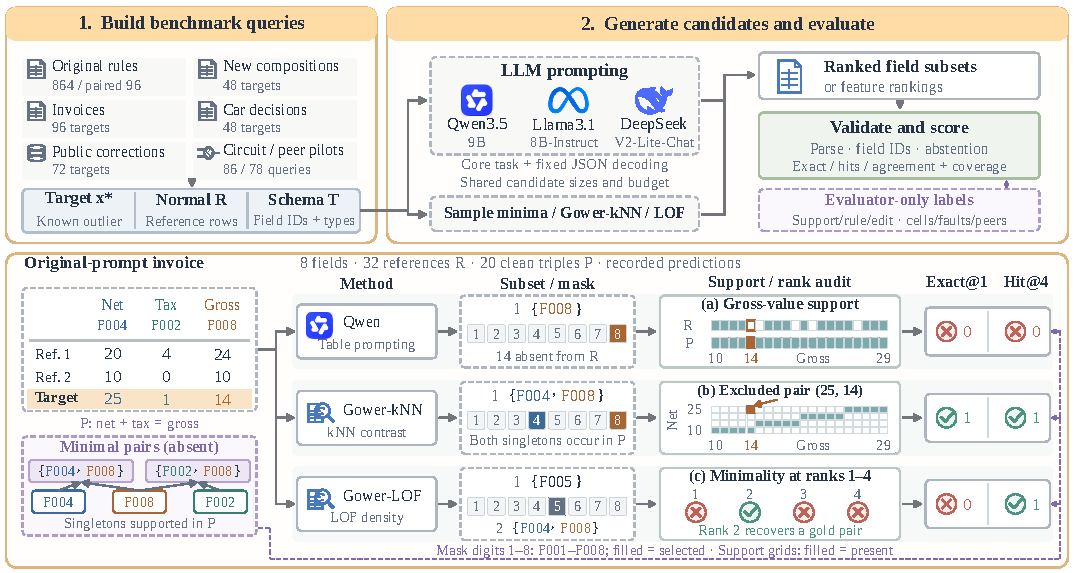
\includegraphics[width=\textwidth]{figures/figure2_overall_framework.pdf}
\caption{Overview of the benchmark. The upper panels separate case construction and hidden labels from the shared query and method comparison. Solid arrows carry inputs or predictions; dashed arrows carry evaluator-only labels. The lower panel follows three evidence paths: exhaustive synthetic labels, circuit-fault labels, and real-table peer references. The primary benchmark ranks up to four subsets; the real-table pilot uses its own three-feature output contract. Each track retains its own metrics and interpretation.}
\label{fig:framework}
\end{figure*}

\section{Benchmark Construction}
\subsection{Procedural benchmark}
We use three random seeds. Each generates 480 cases from 40 rules, with 12 cases per rule. The second and third runs resample values and rotate rule templates across train, development, and test. Each run has 288 test cases; across runs, 864 cases and 38 distinct test templates are evaluated. The eight task families cover rare numeric or categorical values, pairwise and higher-order interactions, conditional patterns, multiple valid explanations, edits that differ from rule fields, and relational violations. Numeric and ordinal domains are small and finite, allowing exhaustive population checks.

Cases have 6, 12, or 24 fields and 8, 16, or 32 normal reference rows. Fields include numeric, binary, categorical, ordinal, date-like, and identifier-like values. Dates and identifiers serve only as distractors. Other distractors include independent noise, a 64-category field, noisy or deterministic proxies, and missing values. These factors are balanced individually, not in every possible combination.

We split by rule template: 8 templates (96 cases) for training, 8 (96) for development, and 24 (288) for testing. No rule appears in more than one split. A method sees only the schema, target, and sampled normal rows. We withhold rule IDs, generator logic, hidden clean rows, and labels. Labels come from exhaustive enumeration of each finite clean population, independently of the sampled references and model outputs. The task is therefore to infer a population property from 8--32 examples.

Each family has five templates and 60 cases; three held-out templates provide 36 test cases per family. The eight families cover distinct rule structures. Numeric marginal rules use a threshold or interval over one numeric or ordinal field; categorical rules mark a category or category set. Pairwise rules use a conjunction, while conditional rules make a signal meaningful only within a context. The multiple-valid family uses a disjunction so either of two singleton fields can be minimal. In the modified-versus-mechanism family, an incidental decoy changes alongside a rule field, separating hidden edit provenance from rule relevance. Relational rules compare two fields through inequality, ordering, a gap, or a sum. Higher-order rules combine three binary or mixed-type conditions using conjunction, parity, or an at-least-$k$ threshold. Thus, the benchmark includes one-field explanations, multi-field interactions, and cases with more than one valid answer. Each family has only three held-out templates, so its individual score is descriptive; factors are balanced marginally, not as a full factorial design.



For each rule, the generator enumerates all assignments to its finite roles and separates clean from anomalous rows. It samples a hidden clean row and a target that satisfies the rule but differs from that clean row. Active roles are mapped to randomly named fields; distractors and normal reference rows are then added. We identify rule fields by checking whether changing a role can change the rule outcome. We find sufficient subsets by checking every full assignment that matches the target on that subset. For support labels, we check whether any clean assignment matches the target projection, including proxy constraints. We retain only subsets with no smaller sufficient subset. Feature names and row and column order are randomized independently of rule roles. This gives exact labels for the finite population, but does not make the sampled reference rows representative by assumption.

Six nuisance settings change distractors while preserving the task label: independent noise, a 64-category field, proxies with 20\% or 40\% reference flips, a deterministic proxy preserved or broken at the target, and a categorical field with independent 15\% missingness. This tests sensitivity to distractors and proxies; it does not test MAR or MNAR missingness.



\subsection{External digital-circuit track}
The digital-circuit package contains four circuits, 64 modified-table/explanation pairs, and 16 original tables. Its labels describe input fields affecting outputs after one logic gate is negated. We checked all 16 zero-noise pairs by matching modified and original rows on their full input vectors. Across 66,834 labeled anomalous rows, every label matched a changed output, each row had one label, and feature names matched the observed output changes. We found no alignment errors.

We sample 64 anomalous rows and create 86 queries by separating rows with multiple changed outputs. Each query uses 16 clean rows from its original truth table, excluding the target's input vector. Methods see all circuit outputs, but may explain only input fields. We withhold labels and fault-generation details. Gold subsets contain 1--12 fields; 47 of 86 contain more than three. Thus, baselines search all nonempty input subsets. This is a narrow binary, single-gate pilot, not general business-table truth.

\subsection{Real-table weak-reference track}
The real-table pilot has 70 queries from nine small ADBench datasets and eight from UCI Lymphography. Five local model families annotate each query. Of 390 responses, 350 are schema-valid and one of those abstains; the remaining 349 valid responses are non-abstentions. In leave-one-model-out evaluation, we remove one model and compare its output with a strict majority of the others' valid, non-abstaining outputs. We leave a case unscored if fewer than two peer outputs are valid or they produce no nonempty majority. Lymphography has only two normal reference rows, and ADBench feature names are opaque. These annotations are not ground truth. We report synthetic, circuit, and real-table results separately because their evidence differs.



\section{Evaluation Protocol}
\subsection{Models and output handling}
The main comparison uses local Qwen3.5-9B, DeepSeek-V2-Lite-Chat, and Llama-3.1-8B-Instruct models with the same prompt and input rows. The prompt requests compact JSON. Decoding is greedy; inputs are capped at 16,384 tokens without truncation, and outputs at 512 tokens. All three models use the same software runtime for the primary comparison, but use one, two, and one 24-GB GPUs, respectively. Latency is therefore not a controlled speed comparison. We test only this direct prompt, not prompts with self-checks, explicit interaction instructions, or tools.

For scoring, we extract the first JSON object. Strict compliance also requires JSON-only output, the requested keys, and evidence fields of no more than 20 words. We do not edit model outputs. Missing, invalid, and empty predictions remain in the denominator and count as misses.

\subsection{Real-table annotation protocol}
The real-table pilot uses a separate prompt and output schema. Each query includes the feature schema, summaries computed from the normal pool, 12 sampled normal rows, and the target row. Source row IDs and class labels are withheld. ADBench fields use opaque IDs because the public files do not preserve names; the UCI Lymphography view provides field names and category descriptions. Models return zero to three feature IDs in ranked order, a deviation direction for each ID, an abstention flag, a confidence value, and a brief uncertainty note. The parser checks the required keys, allowed direction values, ID membership, and the three-ID limit. We retain raw responses and count invalid outputs in the reported validity rates. Confidence and uncertainty notes are not scored as calibrated or faithful evidence.

For leave-one-model-out scoring, the held-out model's nonempty feature set is compared with the strict majority of the other models' valid, non-abstaining feature sets. A query is eligible only when at least two peers respond validly and their outputs yield a nonempty majority. Coverage is the share of valid held-out outputs that are eligible; Jaccard is averaged over eligible comparisons. This protocol measures consistency under a shared prompt and reference sample. Because no independently reviewed feature-level label is available, peer consensus remains a weak reference and cannot establish correctness.

\subsection{Baselines}
All primary baselines receive the same target, schema, and normal rows as the language models. The all-feature control returns every field. The random baseline returns up to four subsets, with subset sizes drawn from the training-set label distribution; it uses no test labels and is averaged over 100 seeds. The univariate baseline returns the four highest-scoring single fields. For numeric and ordinal fields, its score is the larger of empirical rarity and absolute deviation from the median divided by $1.4826\,\mathrm{MAD}$. For other types, it uses empirical rarity.

We also evaluate two mixed-type subspace rankers. They enumerate subsets of one to three fields and use mean Gower distance~\cite{gower1971similarity}. Numeric, ordinal, and date-like values are scaled by their range in the references; categorical, binary, and identifier fields use mismatch distance. A missing-value mismatch has distance one. Gower-kNN compares the target's mean distance to its three nearest references with leave-one-out distances among the normal rows, then returns the four highest-ranked subsets. Gower-LOF uses local outlier factor (LOF) with the same distances and reference-only density estimates~\cite{breunig2000lof}. These are mixed-type adaptations, not canonical subspace implementations. In this test split, all support- and rule-minimal labels contain at most three fields, so the search bound omits no known minimal set. This does not show that three fields are sufficient in other data.

Two oracle controls return the hidden minimal support or rule labels. They use test labels and serve only as upper bounds. We also test SOD and COP adapters~\cite{kriegel2009sod,kriegel2012cop}. Both use scaled numeric/date fields and one-hot categorical, binary, and identifier fields. SOD selects a shared-neighbor subspace; COP uses local PCA and maps its correlation errors back to input fields. These adaptations do not reproduce every option of the original methods. We run M\textsuperscript{2}OE, a single-outlier explainer that returns field choices and a value mask~\cite{angiulli2024m2oe}. We score only its choices because the mask is outside our task. Since it does not rank choices, we compare it using order-independent metrics, not top-one accuracy or reciprocal rank. Minor compatibility edits were required to run its implementation with the available TensorFlow and Keras versions.

RLAX is a close comparator because it ranks subspaces using a margin objective and reinforcement learning~\cite{amirato2026rlax}. We implement a paper-guided adaptation with a PPO policy and rank its candidate subsets. For each query, the known outlier is the positive example and the normal reference rows are split into two disjoint groups. Numeric fields are scaled; categorical fields use mismatch distances. PPO runs for 256 steps and four update epochs per query, fewer than the 2,048 steps and 10 epochs reported for the original method. The target values enter the margin reward, but hidden labels do not. This is a per-query adaptation, not a policy trained across benchmark cases, and we do not claim that it converges to the original setting. Its scores are diagnostic. SHAP-style methods explain a detector score, which our input does not provide~\cite{li2024xadsurvey}.

For the circuit pilot, four controls search every nonempty input subset (up to 14 fields) and return four candidates. This covers the gold-set sizes without using labels to choose subsets. Binary Gower-kNN and Gower-LOF use only target and normal input rows. Two surprisal baselines use observed circuit outputs: one scores the focus output, and one scores the joint output vector, conditional on matching reference values. We also compare each language model with all outputs visible and with only the focus output visible. These paired prompts test the effect of context; they do not give statistical baselines the same input protocol. No baseline uses circuit labels.

\subsection{Research questions and metrics}
We ask five questions: how much the finite references reveal (RQ1), how methods localize the outlier (RQ2), whether their outputs are usable (RQ3), how results change with field order and reference count (RQ4), and whether models agree on real tables (RQ5). The four primary metrics are support sufficiency, exact recovery of a minimal set, Hit@4, and best Jaccard@4. We also report subset size and output validity. Rule labels and support labels are scored separately.

Let $\widehat{\mathcal E}=(S_1,\ldots,S_4)$ be the ranked predictions and $\mathcal G$ the minimal gold alternatives. Sufficiency@1 asks whether $S_1$ contains any gold set. Exact@1 asks whether $S_1$ is a gold set. Hit@4 asks whether any of the first four candidates exactly matches a gold set. Best Jaccard@4 is the largest Jaccard overlap between a top-four candidate and a gold set. We also compute reciprocal rank of the first exact match and Recall@4 over distinct gold alternatives. Invalid, missing, or empty outputs count as misses; duplicates do not increase recall. We report schema validity and strict JSON compliance separately. We do not score free-text evidence or model confidence, so they are not treated as measures of faithfulness or calibration.

For a gold family $\mathcal G$, these measures separate containment from minimal recovery:
\begin{align}
\mathrm{Suff@1} &= \mathbb{I}\!\left[\exists G\in\mathcal G: G\subseteq S_1\right], \\
\mathrm{Exact@1} &= \mathbb{I}[S_1\in\mathcal G], \\
\mathrm{Hit@4} &= \mathbb{I}\!\left[\exists k\leq4: S_k\in\mathcal G\right], \\
\mathrm{Jaccard@4} &= \max_{k\leq4,\,G\in\mathcal G}
\frac{|S_k\cap G|}{|S_k\cup G|}.
\end{align}
Sufficiency rewards any prediction that contains a minimal answer; exact recovery requires equality with one gold alternative. Jaccard gives partial credit but does not replace either measure. We apply the same definitions to support and rule gold sets separately.

We evaluate three seed-specific splits, with 288 test cases per seed and 38 distinct test templates overall. The three models use the same software runtime for the primary comparison. We report each seed and their macro mean. Confidence intervals resample held-out templates, using the same template multiplicities across seeds before averaging. Paired tests compare the three language models with six ranked baselines on four localization metrics and compare model pairs on the same metrics. M\textsuperscript{2}OE is evaluated separately with a matched three-choice budget because its output is not ranked. Random and all-feature controls are descriptive. We report Brier score and 10-bin expected calibration error (ECE) only for valid top-one outputs. A separate text check confirms whether cited field IDs and selected categorical, identifier, or date values appear in the input; it does not test whether the explanation is semantically correct.

Two order probes test sensitivity. In the 96-case probe, Qwen receives reversed field order, reversed reference-row order, both reversals, or permuted feature IDs. We combine these eight contrasts with 12 comparisons of nested reference sets (8, 16, and 32 rows) in one 20-test Holm family. The full order probe tests all three models on 288 cases, each with four independently randomized field orders. We average paired changes within template before inference; seven support and rule metrics form a separate 21-test Holm family. We report validity by condition and compute compactness only on valid outputs. All sensitivity conditions were set before analysis.

We also evaluate Phi-4-mini-instruct on one 288-case split using the same prompt and decoding limits. This descriptive check is excluded from the primary statistical comparisons.

\subsection{Finite-reference support audit}
To measure what the sampled references reveal, we enumerate all feature subsets of size one to three. A subset is sample-absent if the target's values do not appear in any normal reference row. It is sample-minimal if no smaller enumerated subset is sample-absent. We compare these subsets with the population-level labels. This is a diagnostic, not a replacement label or a model score, and it does not assume that models use a literal absence test. We report template-bootstrap intervals and results by field count and reference count.

\section{Results}
\subsection{RQ1: Finite-reference support ambiguity}
\textbf{Finding 1: finite samples create extra explanations.} Across three seeds, sample-minimal subsets exactly matched the population-level labels in only 2 of 864 cases. The other 862 cases had at least one extra subset that appeared minimal in the references. There were 60.93 such extra subsets per case on average (95\% template-cluster interval [57.48,64.39]); 0.863 of population-minimal sets remained sample-minimal. We first average cases within each test template, then average over the 38 test templates. This is an evidence-availability diagnostic, not a model-accuracy score: simple absence in a finite sample is usually insufficient to identify the population label. Figure~\ref{fig:reference-audit} shows the results by field and reference count.

The search contains 41 subsets at six fields, 298 at 12 fields, and 2,324 at 24 fields. At 12 and 24 fields, more references generally retain more population-minimal sets, but also produce more extra minimal-looking subsets. This pattern appears in all six nuisance settings. At 24 fields and 32 references, for example, 95.6\% of population-minimal sets remain sample-minimal, yet there are 233.64 extra candidates per case on average. Reference-count groups are independently generated rather than nested. Minimality is also non-monotone: a false-absence subset can make a larger valid subset appear nonminimal. Counts therefore depend on the candidate universe and are not probabilities that individual explanations are false.

Under the clean-reference assumption, a target projection absent from the full clean population must also be absent from the sample. Sampling can create extra absences, but cannot erase a true population absence. A spurious small subset can then make a larger population-minimal subset appear nonminimal. This is why the reference audit measures label observability rather than model performance.

We also test whether predictions are absent from the visible normal rows. This is a necessary check under our clean-reference assumption, but it does not establish population-level minimality. Qwen's first prediction is sample-absent in 0.911 of cases, and 0.920 of top-four lists contain such a candidate. Yet population exact@1 is 0.425, and 0.486 of its first predictions are sample-absent but not population-minimal. Gower-LOF's first prediction is sample-absent in 0.741 of cases; 0.966 of lists include one, while population Hit@4 is 0.634. These diagnostics do not change the gold labels or main scores. They show that matching the sample does not establish a correct explanation.

\begin{figure*}[t]
\centering
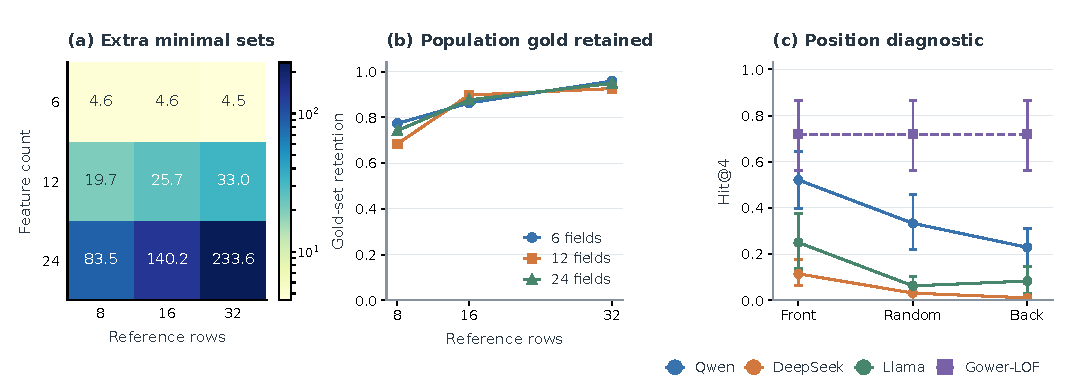
\includegraphics[width=\textwidth]{figures/figure3_reference_and_order_robustness.pdf}
\caption{(a) Extra subsets that appear minimal in the sampled references, by field and reference count; (b) fraction of population-minimal sets retained in the sample; and (c) score changes after randomizing field order. Panel (c) shows four localization metrics with 95\% template/order bootstrap intervals; zero means no change. Reference-count groups are independently generated, not nested. Panels (a,b) are descriptive; panel (c) reports paired sensitivity, not a method ranking.}
\label{fig:reference-audit}
\end{figure*}

\subsection{RQ2: Localization against an expanded baseline suite}
\begin{table*}[t]
\centering\footnotesize
\caption{Localization under a fixed input protocol. Entries are three-seed macro means. Bold marks the best non-control method in each localization column; all-feature sufficiency is a trivial upper bound. Invalid outputs count as misses. Selected-field fraction is computed on valid outputs and is descriptive.}
\setlength{\tabcolsep}{2.8pt}
\renewcommand{\arraystretch}{1.15}
\begin{tabular*}{\textwidth}{@{\extracolsep{\fill}}|c|l|c|rrrr|rrr|r|}
\hline
\multicolumn{2}{|c|}{Methods} & \multirow{2}{*}{Input} & \multicolumn{4}{c|}{Population-support labels ($\uparrow$)} & \multicolumn{3}{c|}{Rule labels ($\uparrow$)} & \multirow{2}{*}{\shortstack{Selected\\fraction}} \\
\cline{1-2}\cline{4-10}
Group & Method & & Suff.@1 & Exact@1 & Hit@4 & Jaccard@4 & Suff.@1 & Exact@1 & Hit@4 & \\
\hline
\multirow{3}{*}{\rotatebox{90}{\scriptsize LMs}} & Qwen3.5-9B & \multirow{11}{*}{\rotatebox{90}{Fixed $T$, $x^*$, $R$}} & \textbf{0.714} & 0.425 & 0.451 & 0.659 & \textbf{0.684} & 0.403 & 0.426 & 0.207 \\
& DeepSeek-V2-Lite-Chat & & 0.429 & 0.125 & 0.145 & 0.315 & 0.407 & 0.115 & 0.134 & 0.371 \\
& Llama-3.1-8B-Instruct & & 0.394 & 0.152 & 0.177 & 0.383 & 0.380 & 0.140 & 0.163 & 0.199 \\
\cline{1-2}\cline{4-11}
\multirow{3}{*}{\rotatebox{90}{\scriptsize Rankers}} & Gower-LOF & & 0.545 & \textbf{0.517} & \textbf{0.634} & \textbf{0.759} & 0.528 & \textbf{0.500} & \textbf{0.603} & 0.181 \\
& Gower-kNN & & 0.608 & 0.400 & 0.495 & 0.684 & 0.583 & 0.383 & 0.476 & 0.229 \\
& RLAX adaptation & & 0.507 & 0.417 & 0.495 & 0.692 & 0.468 & 0.382 & 0.464 & 0.234 \\
\cline{1-2}\cline{4-11}
\multirow{3}{*}{\rotatebox{90}{\scriptsize Controls}} & Top-four univariate & & 0.155 & 0.155 & 0.398 & 0.547 & 0.140 & 0.140 & 0.392 & 0.097 \\
& Random size prior & & 0.117 & 0.038 & 0.132 & 0.353 & 0.102 & 0.032 & 0.115 & 0.162 \\
& All features & & 1.000 & 0.000 & 0.000 & 0.155 & 1.000 & 0.000 & 0.000 & 1.000 \\
\cline{1-2}\cline{4-11}
\multirow{2}{*}{\rotatebox{90}{\scriptsize Adapt}} & SOD adaptation & & 0.512 & 0.000 & 0.000 & 0.145 & 0.500 & 0.000 & 0.000 & 0.558 \\
& COP adaptation & & 0.005 & 0.005 & 0.013 & 0.131 & 0.005 & 0.005 & 0.012 & 0.242 \\
\hline
\end{tabular*}
\renewcommand{\arraystretch}{1.0}
\label{tab:main}
\end{table*}

\begin{figure*}[t]
\centering
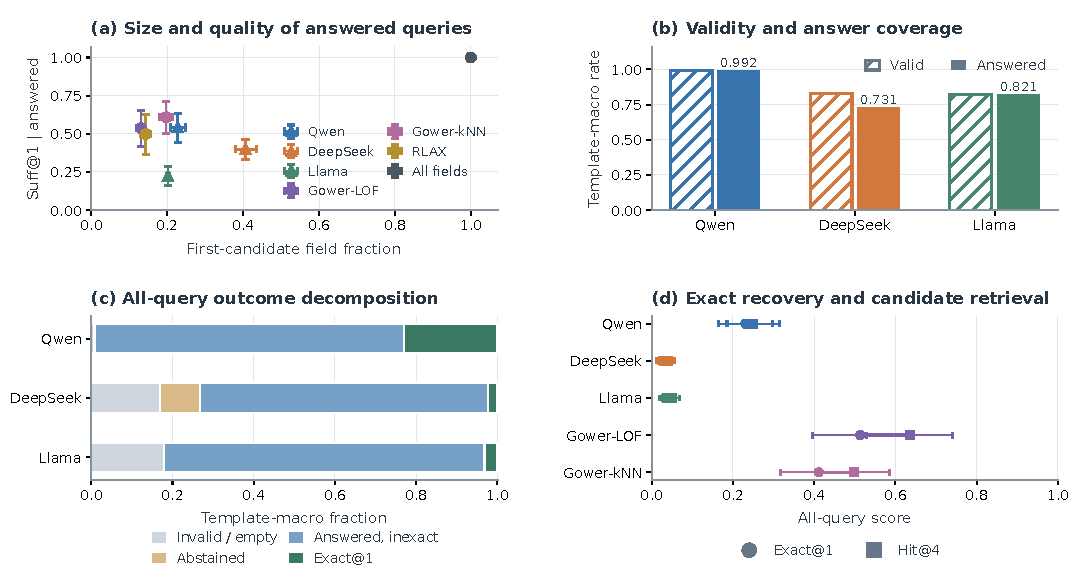
\includegraphics[width=\textwidth]{figures/figure2_sufficiency_compactness_validity.pdf}
\caption{Localization and output behavior. (a) Support sufficiency versus selected-field fraction for the language models, main subspace rankers, and all-feature control; bars show template-bootstrap intervals. (b) Sufficiency with invalid responses counted as misses versus sufficiency on valid responses. (c) Schema-valid and strict-JSON rates. (d) Mean and 95th-percentile latency. Tokenizers and GPU counts differ across models, so latency is descriptive.}
\label{fig:pareto}
\end{figure*}

\textbf{Finding 2: the preferred method depends on the metric.} Sufficiency rises as subsets get larger, so it must be read together with subset size. The all-feature control reaches sufficiency 1.000 by definition but selects every field and never recovers a minimal set. Among the language models, DeepSeek has slightly higher sufficiency than Llama (0.429 versus 0.394), but also returns broader valid subsets (field fractions 0.371 versus 0.199). Qwen has the highest model sufficiency@1 (0.714). Gower-LOF has the strongest exact@1 (0.517), Hit@4 (0.634), and best Jaccard@4 (0.759).

We test paired differences over 38 template clusters using 20,000 sign flips and Holm correction. In the 78-comparison family, Qwen's sufficiency is 0.156 higher than Gower-LOF's (95\% CI [0.102,0.211], adjusted $p=0.0039$). Gower-LOF leads Qwen on Hit@4 by 0.202 and Jaccard by 0.115 (both adjusted $p=0.0039$); their exact@1 difference is not significant ($p=0.137$). Qwen and Gower-kNN do not differ on the three retrieval metrics, but Qwen has higher sufficiency (+0.098, adjusted $p=0.0081$). The RLAX adaptation shows no detected difference from Qwen on retrieval, while Qwen has higher sufficiency (+0.196, adjusted $p=0.0039$). This does not establish equivalence; the short RLAX run may be under-optimized. Table averages weight cases within each seed, while paired tests weight templates equally, so paired effects can differ from differences between table entries.

In a separate 12-comparison family, Qwen outperforms DeepSeek and Llama on all four primary measures (adjusted $p=0.0006$). DeepSeek and Llama do not differ on sufficiency, exact@1, or Hit@4 after correction; Llama's best Jaccard is higher by 0.065 (adjusted $p=0.0018$). These tests are exploratory, and a nonsignificant result is not evidence that two methods are equivalent.

SOD often returns broad subsets (mean size 7.55) and has no exact or Hit@4 matches. COP returns smaller subsets (mean size 2.50) but has near-zero sufficiency. These results describe our adapters, not canonical SOD or COP performance. The top-four univariate baseline reaches Hit@4 of 0.398 and Jaccard of 0.547, showing that marginal rarity alone recovers some subset overlap. On the separate rule target, Qwen leads sufficiency@1 (0.684), while Gower-LOF leads exact@1 (0.500) and Hit@4 (0.603). Support, rule, and mechanism labels therefore measure different targets.

M\textsuperscript{2}OE returns an unordered choice set, so we compare it separately using three choices. Hit@3 / best Jaccard@3 are 0.450/0.659 for Qwen, 0.142/0.311 for DeepSeek, 0.175/0.381 for Llama, and 0.000/0.192 for M\textsuperscript{2}OE. Qwen exceeds M\textsuperscript{2}OE by 0.439 in Hit@3 (95\% CI [0.362,0.519]) and 0.462 in Jaccard (95\% CI [0.407,0.515]); both adjusted $p=0.0039$. This comparison scores only field choices, not the value mask or a ranked-list objective.

We also score hidden edit provenance, which is not shown to methods. At four candidates, Gower-LOF exactly recovers the directly edited fields in 0.451 of cases. RLAX has the highest direct-field recall (0.787). Qwen's exact recovery is 0.281, with direct-field recall 0.740 and changed-value recall 0.742. RLAX and Gower-LOF have changed-value recall of 0.785 and 0.775. The all-feature control covers every field but never exactly matches the edit set. This is a secondary provenance analysis, not explanation accuracy: the visible prompt does not reveal which value was intentionally changed.

\subsection{RQ3: Output validity and task-family profile}
\textbf{Finding 3: output validity changes the effective score.} Across 864 runs, schema-valid rates are 0.991 for Qwen, 0.806 for DeepSeek, and 0.817 for Llama. Strict JSON-contract rates are lower: 0.988, 0.387, and 0.661. Invalid-response counts are 8, 168, and 158. Most DeepSeek and Llama failures reached the 512-token output limit; other failures involved malformed output or schema violations. We report scores both for parseable responses and for all runs, where invalid outputs count as misses.

Among valid responses, sufficiency@1 is 0.721 for Qwen, 0.533 for DeepSeek, and 0.481 for Llama. Counting invalid responses as misses lowers these scores to 0.714, 0.429, and 0.394 (Figure~\ref{fig:pareto}). Llama's compact outputs mostly contain two fields (1,556 of 1,635 candidates), but this does not mean they localize the anomaly better. Self-reported confidence is poorly aligned with exact recovery: mean confidence is 0.952, 0.852, and 0.804; Brier scores are 0.514, 0.626, and 0.532; and 10-bin ECE is 0.523, 0.697, and 0.619. The input-token check confirms only that cited values appear in the prompt; it does not verify the explanation. We did not conduct a human faithfulness review.
Task-family, field-count, reference-count, and nuisance analyses are descriptive because each family has only three test templates and the other groups are not paired interventions. The only missingness test is independent 15\% missingness in one categorical distractor; we do not test MAR or MNAR. On one split, Phi-4-mini-instruct has sufficiency@1 0.441, exact@1 0.135, Hit@4 0.160, and Jaccard 0.376 from 271 structured outputs. This result is descriptive and excluded from paired tests. Its real-table Jaccard of 0.467 measures peer agreement, so it is not comparable to its synthetic Hit@4.

Latency includes inference and parsing but excludes model loading. Mean prompt lengths differ by tokenizer (6,565 tokens for Qwen, 6,599 for DeepSeek, and 4,839 for Llama), and the models use different numbers of GPUs. The latency plot is therefore descriptive, not a controlled speed ranking. We did not measure energy or monetary cost.



\subsection{RQ4: Order and reference-count robustness}
\textbf{Finding 4: field order affects localization.} The full field-order test uses one 288-case split with 24 templates and four randomized field orders per case. All three models score lower after randomization. Across the four primary metrics, paired changes range from -0.076 to -0.202; rule-sufficiency, exact, and Hit@4 changes are also negative. All 21 support/rule comparisons pass Holm correction ($p_{adj}=0.0010$--$0.0084$). Output validity changes little across conditions. The result applies to this split and prompt only. Baselines were not rerun with shuffled fields, and RLAX uses field position in its input state.

A separate Qwen probe uses 96 cases from the same 24 templates. Reversing field order lowers Hit@4 by 0.354 (95\% CI [-0.448,-0.260]) and best Jaccard by 0.346 ([-0.413,-0.271]); both survive the 20-test Holm correction ($p_{adj}=0.001$). Reversing both fields and references lowers the same metrics by 0.333 and 0.335. Reference-row order and opaque field-ID changes show no corrected effect. This fixed-reversal probe is separate from the full randomized-order test.

For nested reference sets, Qwen's Hit@4 / Jaccard is 0.396/0.608 with 8 rows, 0.531/0.700 with 16, and 0.521/0.662 with 32. The 16-versus-8 increases do not survive correction ($p_{adj}=0.242$ and 0.202), and the 32-versus-16 changes are near zero. Three of 96 outputs are invalid at 32 rows, including two input-limit failures. The 20 planned contrasts were not preregistered. Both 96-case probes use one model; the larger order test uses one held-out split.

\subsection{RQ5: Real-table weak-reference agreement}
\textbf{Finding 5: real-table consensus depends on coverage.} Table~\ref{tab:lomo} reports agreement with the other models' strict-majority feature set. Phi-4-mini-instruct has the highest mean Jaccard estimate (0.467) and DeepSeek the lowest (0.330), but the dataset-cluster intervals overlap and we do not test a ranking. Intervals resample the ten table datasets as clusters. The 78 queries combine 70 ADBench cases with eight Lymphography cases, so the estimate is not a homogeneous natural-table result. Agreement depends on valid outputs and peer consensus, and may reflect shared model, prompt, or training-data biases. It measures agreement, not explanation truth.

Figure~\ref{fig:intro-sample-gap} also illustrates how the weak reference is constructed. All five parsed responses for C0035 are valid and non-abstaining. F001 appears in five responses, F002 and F005 in four each, and F007 in two. Holding out any one model leaves the majority set \{F001, F002, F005\}. Qwen and Llama each obtain Jaccard 0.500, whereas DeepSeek, Gemma, and Phi obtain 1.000. These are agreements on one shared input; they provide no independent reason to accept the majority fields as correct or to reject F007. The example motivates retaining raw rankings and eligibility records alongside pooled means: consensus can hide a disputed field even when every output passes the schema.

Agreement also varies across datasets. Averaging the available held-out-model estimates within each dataset gives mean Jaccard values from 0.107 on Hepatitis to 0.569 on Vertebral; these are descriptive summaries, not accuracy estimates. DeepSeek contributes no valid Stamps outputs, and the Lymphography queries share only two normal references. Both the number of eligible comparisons and the peer set therefore change across datasets. The pooled table is useful as a protocol summary, while per-dataset scores show how strongly consensus can depend on the table and on model coverage.

\begin{table*}[t]
\centering\footnotesize
\caption{Leave-one-model-out evaluation on 78 real-table queries. Coverage is the eligible count divided by the valid, non-abstaining held-out count. Jaccard measures agreement with the peers' strict-majority set; it is not feature-level accuracy.}
\setlength{\tabcolsep}{5pt}
\renewcommand{\arraystretch}{1.12}
\begin{tabular*}{\textwidth}{@{\extracolsep{\fill}}|l|rr|rr|}
\hline
\multirow{2}{*}{Held-out model} & \multicolumn{2}{c|}{Output / reference coverage} & \multicolumn{2}{c|}{Peer-agreement measures} \\
\cline{2-5}
 & Valid outputs & Eligible comparisons & Coverage & Mean Jaccard \\
\hline
DeepSeek-V2-Lite-Chat & 44 & 41 & 0.932 & 0.330 \\
Gemma-3-4B-it & 78 & 70 & 0.897 & 0.459 \\
Llama-3.1-8B-Instruct & 78 & 74 & 0.949 & 0.393 \\
Phi-4-mini-instruct & 72 & 68 & 0.944 & 0.467 \\
Qwen3.5-9B & 77 & 73 & 0.948 & 0.337 \\
\hline
\end{tabular*}
\renewcommand{\arraystretch}{1.0}
\label{tab:lomo}
\end{table*}

\subsection{External digital-circuit pilot}
The circuit pilot has 86 focus-output queries from four circuit pairs and 66,834 labeled anomalous rows. Gold sets contain 1--12 input fields, and 47 of 86 have more than three. We therefore emphasize overlap (Jaccard and field recall) rather than exact match. The candidate budget is four subsets; it does not limit fields per subset. Invalid, missing, or abstained outputs count as misses. Because methods see different information, we report descriptive scores without cross-method ranking tests. Qwen has one exact Hit@4 (0.012); DeepSeek and Llama have none. Valid-output rates are 0.988, 0.186, and 0.233. Best Jaccard@4 is 0.358 for Qwen, 0.449 for Gower-kNN, and 0.423 for conditional-output surprisal. Field-recall@4 is 0.760 for Qwen, 0.744 for Gower-kNN, and 0.606 for surprisal; intervals resample 16 circuit-pair clusters.

When we compare prompts with all circuit outputs against prompts showing only the focus output, no model changes on exact@1 or Hit@4 after correction. Qwen's best Jaccard increases by 0.096 (95\% circuit-pair interval [0.045,0.146], adjusted $p=0.028$ across nine tests); DeepSeek and Llama show no corrected change. This tests context within each model. The narrow, single-gate setting does not establish performance on business tables.

\section{Discussion}
\subsection{The metrics answer different questions}
The primary comparison shows that a high sufficiency score is not enough. A large subset has more chances to contain a sufficient explanation, as the all-feature control demonstrates. Exact@1 asks whether the first answer is one of the minimal explanations; Hit@4 asks whether the method ranks any valid alternative near the top; Jaccard measures partial overlap. A reviewer may value different properties depending on whether the task is triage, rule inspection, or audit. Reporting these measures separately makes the tradeoff visible. In our results, Qwen is strongest on support sufficiency, while Gower-LOF leads exact recovery and retrieval. These results compare methods on this benchmark; they do not establish that language models or rankers are generally superior.

The gap between sufficiency@1 and exact@1 makes this distinction concrete. For Qwen, the scores are 0.714 and 0.425; for Gower-LOF, they are 0.545 and 0.517. A sufficient superset can describe the target under our label definition while still naming more fields than a minimal answer. The gap is descriptive rather than a separate error rate because cases can have multiple minimal alternatives and the metrics answer different questions. A shortlist for investigation may favor coverage, whereas a compact audit trail may favor exact minimal recovery. We do not evaluate these possible uses with human analysts.

\subsection{The reference sample is part of the task}
The synthetic audit establishes a distinction between what the full clean population makes true and what a small reference sample happens to show. A target projection can be absent from every supplied reference row simply because only 8--32 rows are observed. As a result, a system that returns every sample-absent subset may produce many plausible-looking but nonminimal candidates. This concern is more than a property of one explanation algorithm: it is a property of the evidence available to any method. Future evaluations should therefore state whether labels refer to the full population, observed sample, or an expert judgment, and should not treat these targets as interchangeable.

Candidate granularity also limits what can be inferred across tracks. Every minimal synthetic support and rule set in the test split has at most three fields, so the one-to-three-field ranker search covers that gold space. Circuit labels contain up to 12 fields, with 47 of 86 queries above three fields; the circuit controls therefore search all nonempty input subsets. The main benchmark supports a controlled comparison within its stated candidate universe, while the circuit pilot asks whether methods can overlap with much larger fault-specific sets under a different input protocol. Their scores should remain separate.

\subsection{Order and external evidence require careful interpretation}
The field-order test shows that equivalent information presented in a different order can change model outputs. This motivates order perturbation tests when a method reads serialized tables or schemas. Our test does not establish general order sensitivity across prompts, datasets, or models. The circuit pilot adds examples with fault-specific feature labels, but covers only binary single-gate faults. The real-table pilot adds examples from natural datasets, but it has no trusted feature-level labels. We therefore keep both pilots separate from the primary scores. Together, they identify practical evaluation needs; they do not replace broader, independently labeled studies.

\subsection{Recommendations for future evaluations}
The results suggest four reporting practices. \textbf{Specify the label universe.} State whether an explanation is judged against the full clean population, the observed sample, or expert review. Distinguish descriptive support, rule-related fields, and direct edits so that users can tell whether a benchmark asks for a row description, a generating rule, or edit provenance.

\textbf{Measure sufficiency and minimality together.} Report selected-field size, exact recovery, and a ranked-list metric. Retain multiple minimal alternatives in the gold family. Include all-field and univariate controls: the former exposes the trivial route to high sufficiency, while the latter tests whether a complex method improves on marginal rarity. These controls clarify the practical meaning of a gain.

\textbf{Report validity and stability.} Give all-query scores with invalid responses counted as misses, alongside valid-only diagnostics. Record the output contract, decoding limits, and parsing rules. Perturb field order and reference rows; account for shared templates or datasets in uncertainty estimates. Runtime comparisons should use matched hardware and include the same inference and parsing stages.

\textbf{Match claims to evidence.} Keep exhaustive synthetic truth, circuit-fault truth, and real-table peer agreement distinct. A stronger real-table benchmark requires independently reviewed feature-level labels and an explicit policy for alternative explanations. Expert assessment of usefulness would complement localization scores, especially when a broad shortlist and a minimal audit trail have different operational value.

\section{Related Work}
Table~\ref{tab:related-work} summarizes neighboring settings by target, output, and source of evaluation evidence. It is a task comparison, not a claim that the listed systems are interchangeable or directly comparable.

\begin{table*}[t]
\centering\scriptsize
\caption{A unified task-level view of neighboring work. A checkmark identifies a primary target in this taxonomy; a dash denotes a different focus, not absence of a software capability. ``Fault'' includes integrity errors and injected faults. ``Support'' means population-minimal descriptive support.}
\setlength{\tabcolsep}{3.3pt}
\renewcommand{\arraystretch}{1.27}
\begin{tabularx}{\textwidth}{|c|>{\raggedright\arraybackslash}p{1.75cm}|>{\raggedright\arraybackslash}X|c|c|c|c|c|c|}
\hline
\multirow{2}{*}{Category} & \multirow{2}{*}{Task / idea} & \multirow{2}{*}{Representative work} & \multicolumn{6}{c|}{Primary object of evaluation or explanation} \\
\cline{4-9}
 & & & Row & Score & Subspace & Group & Fault & Support \\
\hline
Model & Score attribution & Shapley explanation; CAIT~\cite{kluttermann2024shapley,mok2025cait} & -- & $\checkmark$ & -- & -- & -- & -- \\
\hline
\multirow{3}{*}{Data} & Outlier subspaces & LookOut, ABOD, SOD, COP~\cite{gupta2018lookout,kriegel2008abod,kriegel2009sod,kriegel2012cop} & -- & -- & $\checkmark$ & -- & -- & -- \\
\cline{2-9}
 & Aggregate diagnosis & Adtributor, iDice, HotSpot, Squeeze~\cite{bhagwan2014adtributor,lin2016idice,sun2018hotspot,li2019squeeze} & -- & -- & -- & $\checkmark$ & -- & -- \\
\cline{2-9}
 & Data cleaning & HoloClean; AutoDCWorkflow~\cite{rekatsinas2017holoclean,li2025autodcworkflow} & -- & -- & -- & -- & $\checkmark$ & -- \\
\hline
\multirow{3}{*}{Evaluation} & Anomaly benchmarks & ADBench, TABARD, RADAR~\cite{han2022adbench,choudhury2025tabard,gu2025radar} & $\checkmark$ & -- & -- & -- & $\checkmark$ & -- \\
\cline{2-9}
 & Fault-label studies & Ground-truth anomaly explanations; gate-negation circuits~\cite{antwarg2024groundtruth,myrtakis2021comparative} & -- & -- & $\checkmark$ & -- & $\checkmark$ & -- \\
\cline{2-9}
 & Minimal-set benchmark & This study: known outlier + finite references & -- & -- & $\checkmark$ & -- & -- & $\checkmark$ \\
\hline
\end{tabularx}
\renewcommand{\arraystretch}{1.0}
\label{tab:related-work}
\end{table*}

\subsection{Table anomaly benchmarks and explanations}
Surveys distinguish explanations of a supplied instance from explanations of a detector score~\cite{panjei2022survey,li2024xadsurvey}. Our task receives a known outlier but no score. CAIT and Shapley-based feature-bagging methods explain detector behavior~\cite{mok2025cait,kluttermann2024shapley}; ADBench, TABARD, RADAR, AnTBench, and SEC-FinTables evaluate row detection, data quality, or table-question-answering failures, rather than population-minimal feature sets~\cite{han2022adbench,choudhury2025tabard,gu2025radar,wei2026antbench,ke2026secfintables}. Gate-negation studies provide feature labels for a narrow circuit fault family~\cite{antwarg2024groundtruth,myrtakis2021comparative}. Aggregate systems such as Adtributor, R-Adtributor, iDice, HotSpot, Squeeze, and PSqueeze explain groups or metric changes, not one supplied row~\cite{bhagwan2014adtributor,persson2018radtributor,lin2016idice,sun2018hotspot,li2019squeeze,li2023psqueeze}. Table~\ref{tab:related-work} summarizes these differences.

The evaluation target determines what counts as a correct answer. A faithful score attribution need not be a minimal description of a row; an aggregate segment and a repaired cell answer different questions again. Our labels make this distinction explicit: population support, rule sufficiency, rule-related fields, and hidden edits remain separate. Multiple valid subsets are retained instead of choosing one arbitrary answer. Exhaustive synthetic labels support controlled comparisons, circuit labels support fault-specific claims, and peer consensus provides an agreement measure for real tables. Table~\ref{tab:related-work} therefore organizes neighboring tasks by their primary target rather than suggesting a shared leaderboard.

RLAX ranks subspaces using reinforcement learning; our adaptation trains a separate policy per case and is not a canonical reproduction~\cite{amirato2026rlax}. M\textsuperscript{2}OE also receives a known outlier and normal references, but returns field choices with a value mask for possible repair; we evaluate only its field choices~\cite{angiulli2024m2oe}. Data-engineering systems explain aggregate outliers, learn constraints, or detect and repair integrity violations~\cite{wu2013scorpion,chen2025autotest,chu2013holistic,rekatsinas2017holoclean,li2025autodcworkflow}. ABOD, SOD, COP, and high-contrast projection methods motivate subspace analysis, but typically return scores or detector-focused subspaces~\cite{kriegel2008abod,kriegel2009sod,kriegel2012cop,muller2011subspace,keller2012hics}. RMKN and EAMOD improve outlier scoring with learned kernels; our benchmark begins after a row has been flagged~\cite{wang2024rmkn,wang2024eamod}. Across these settings, our contribution is the evaluation of ranked field subsets against separate support, rule, mechanism, and edit labels.

\section{Artifact and Reproducibility}
The accompanying artifact contains the benchmark generator, prompts, labels, raw model outputs, parsers, baseline predictions, per-case scores, and SHA-256 manifests. It records model hashes, decoding limits, seeds, failures, and analysis settings; model weights are excluded. The main comparison and figures can be regenerated from the artifact. The anonymous artifact link is a placeholder and has not yet been hosted: \url{https://example.org/anonymous-artifact-link-pending}.

The original runs used Transformers 5.15.0 and PyTorch 2.13.0+cu130. The shared-runtime replications, circuit pilot, and order tests used Transformers 5.22.1 and PyTorch 2.14.1+cu126 on RTX 3090 GPUs. Generator seeds are 20261106--20261108; field-order permutations use seeds 1001--1004 and the nested bootstrap uses seed 1005. We use 2,000 template-bootstrap replicates for confidence intervals and 20,000 sign flips for paired tests. The randomized-order analysis applies a separate 21-test Holm correction. Compactness is calculated only for valid outputs.

\textbf{Figure provenance.} Figure~\ref{fig:intro-sample-gap} is reconstructed from recorded Pima values, reference indices, and model responses; no new inference is required.

\section{Limitations}
\begin{enumerate}
  \item One synthetic generator with 40 rules and 38 observed test templates cannot cover the diversity of real tables.
  \item Labels use the complete synthetic population, while methods see 8--32 references; sample absence can therefore be misleading.
  \item Dates and identifiers are only distractors; their role in generating anomalies remains untested.
  \item Missingness is limited to independent 15\% missingness in one categorical distractor; MAR and MNAR patterns remain untested.
  \item The Gower, SOD, COP, and RLAX scores apply to task-specific adaptations.
  \item The circuit pilot covers 86 binary, single-gate queries. It does not represent general business-table faults.
  \item Real-table evaluation uses peer-model agreement because feature-level truth is unavailable. Agreement among related models is not accuracy.
  \item The field-order experiment uses one 288-case split and one prompt. It cannot establish robustness across prompts or datasets.
  \item Domain experts did not assess explanation faithfulness, clarity, or usefulness.
  \item We did not measure review time, repair quality, energy use, or monetary cost.
  \item Models used different GPU counts and tokenizers. Latency is descriptive, not a controlled speed comparison.
  \item Opaque feature names reduce direct clues but cannot rule out exposure to the benchmark during model pretraining.
\end{enumerate}

\section{Conclusion}
Finite references produced extra minimal-looking subsets in 862 of 864 cases, and field-order randomization reduced all three language models' scores. Qwen led support sufficiency; Gower-LOF led exact and ranked retrieval. The all-feature control demonstrated the need to report subset size. Broader generators, independently labeled real tables, expert review, and external reproduction remain necessary.

\section*{Acknowledgments and AI Use Disclosure}
OpenAI Codex assisted with code, analysis, figures, and drafting. Outputs were generated by Qwen3.5-9B, DeepSeek-V2-Lite-Chat, Llama-3.1-8B-Instruct, Phi-4-mini-instruct, and Gemma-3-4B-it. The author is responsible for all claims, citations, data, and results.

\bibliographystyle{IEEEtran}
\bibliography{phase_d_references}
\end{document}
